\documentclass{beamer}
%
% Choose how your presentation looks.
%
% For more themes, color themes and font themes, see:
% http://deic.uab.es/~iblanes/beamer_gallery/index_by_theme.html
%
\mode<presentation>
{
  \usetheme{AnnArbor}      % or try Darmstadt, Madrid, Warsaw, ...
  \usecolortheme{default} % or try albatross, beaver, crane, ...
  \usefonttheme{default}  % or try serif, structurebold, ...
  \setbeamertemplate{navigation symbols}{}
  \setbeamertemplate{caption}[numbered]
} 

\usepackage[english]{babel}
\usepackage[utf8x]{inputenc}
\usepackage{hyperref}
\hypersetup{colorlinks=true}
\usepackage{graphicx}
\graphicspath{{./figures/}}
\usepackage{caption}
\usepackage{subcaption}
\usepackage{amsmath}

\title[Bayesian Neural Networks]{
Bayesian Neural Networks
}
%\author{Victor Verma}
\author[Victor Verma]{Victor Verma}
\institute[]{Hot Ideas in Machine Learning Reading Group, University of Michigan}
\date{7/15/22}

\begin{document}

\begin{frame}
  \titlepage
\end{frame}

% Uncomment these lines for an automatically generated outline.
%\begin{frame}{Outline}
%  \tableofcontents
%\end{frame}

%\section{Introduction}

\begin{frame}{Generalization in Bayesian deep learning}
    "Being Bayesian" can improve
    \begin{itemize}
        \item Predictive accuracy
        \item Generalization performance
    \end{itemize}
\end{frame}

\begin{frame}{Sharp vs flat minima}
    A minimum of a loss function can be \textbf{sharp} or \textbf{flat}.
    \begin{itemize}
        \item At a sharp minimum, the function has a narrow, deep hole (Fig.~\ref{fig:sharp_minimum}).
        \item At a flat minimum, it has a broad, shallow hole (Fig.~\ref{fig:flat_minimum}).
    \end{itemize}
    
    \begin{figure}
        \centering
        \begin{subfigure}[b]{0.4\textwidth}
            \centering
            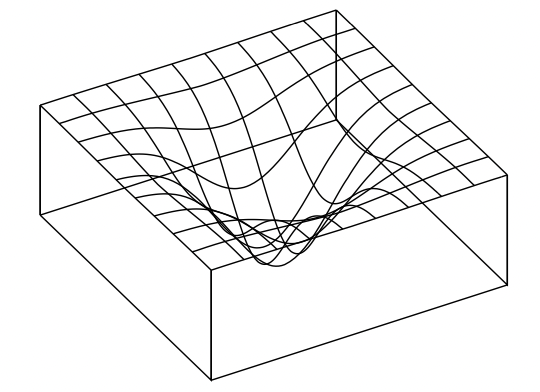
\includegraphics[width=\textwidth]{sharp_minimum}
            \caption{A sharp minimum}
            \label{fig:sharp_minimum}
        \end{subfigure}
        \begin{subfigure}[b]{0.4\textwidth}
            \centering
            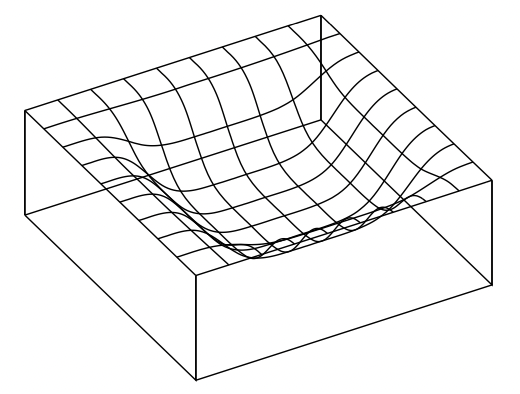
\includegraphics[width=\textwidth]{flat_minimum}
            \caption{A flat minimum}
            \label{fig:flat_minimum}
        \end{subfigure}
        \caption{Sharp and flat minima}
        \label{fig:sharp_and_flat_minima}
    \end{figure}
\end{frame}

\begin{frame}{Sharp vs flat minima}
    Flat minima are preferable to sharp minima for two reasons:
    \begin{itemize}
        \item A sharp minimum corresponds to a tiny loss, which is typically caused by overfitting.
        \item Flat minima are more robust and generalize better. This can seen in two ways:
            \begin{itemize}
                \item A flat minimum corresponds to a region in parameter space with high posterior uncertainty; samples from the region don't memorize irrelevant details of the training set.
                \item A flat minimum has a short description length, i.e., few bits are needed to specify its location. This results in better generalization.
            \end{itemize}
    \end{itemize}
\end{frame}

\begin{frame}{Sharp vs flat minima}
    SGD (Stochastic Gradient Descent) tends to avoid sharp minima:
    \begin{itemize}
        \item A sharp minimum is in a region $\mathcal{A}$ of low evidence.
        \item The evidence for $\mathcal{A}$ is proportional to $\int_{\mathcal{A}} e^{-\mathcal{L}(\boldsymbol{\theta})}\,d\boldsymbol{\theta}$, so this integral is small.
        \item The integral is proportional to SGD's probability of entering $\mathcal{A}$, so SGD is unlikely to enter $\mathcal{A}$.
    \end{itemize}
    This property is due to SGD's use of noise.
\end{frame}

\begin{frame}{Effective dimensionality of a model}
    The \textbf{effective dimensionality} of a model reflects how many well-determined parameters it has. It is defined as
    \begin{equation*}
        N_{\text{eff}}(\boldsymbol{H}, c) = \sum_{i = 1}^k \frac{\lambda_i}{\lambda_i + c},
    \end{equation*}
    where $\boldsymbol{H}$ is the Hessian of the loss at the appropriate local mode, $\lambda_1, \ldots, \lambda_k$ are $\boldsymbol{H}$'s eigenvalues, and $c$ is a regularization constant.
    
    \medskip
    
    A low effective dimensionality implies that significant compression is possible. Also, the effective dimensionality is a good proxy for generalization.
\end{frame}

\begin{frame}{Effective dimensionality of a model}
    Fig.~\ref{fig:effective_dimensionality_and_test_loss} illustrates the last point on the previous slide. For CNNs with near-zero training loss, the pattern in the test loss closely resembles that in the effective dimensionality.
    \begin{figure}
        \centering
        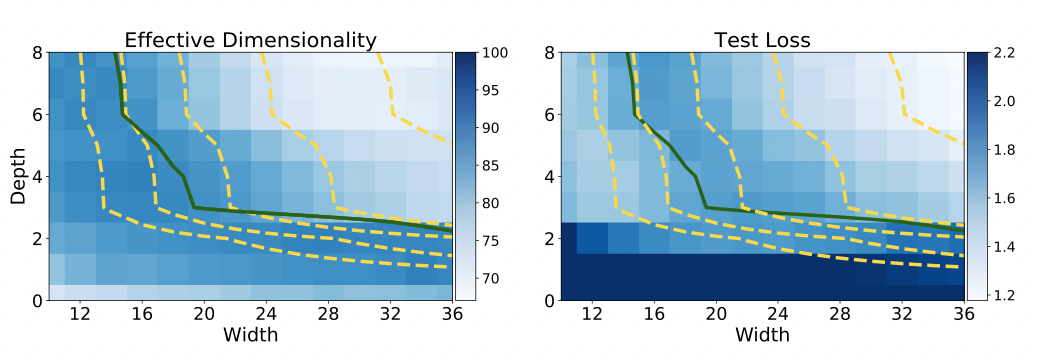
\includegraphics[width=\textwidth]{effective_dimensionality_and_test_loss}
        \caption{Effective dimensionality and test loss for various CNNs trained on the CIFAR-100 image dataset. CNNs above the green curve have near-zero training loss. CNNs on the same yellow curve have the same number of parameters.}
        \label{fig:effective_dimensionality_and_test_loss}
    \end{figure}    
\end{frame}

\end{document}